\section{Understanding The Packet}

\begin{frame}
   {What Are We Sending}
      \begin{itemize}
	 \item Payload
         \item Encapsulation
	 \item Header Sections
	 \item TCP/IP and OSI Models
      \end{itemize}


\end{frame}

\cprotect\note{

}

\begin{frame}
   {Encapsulation}
      \begin{itemize}
         \item Variable size payload
	 \item Adding parameters for wide range of recipients
	 \item Unencapsulated by recipient network stack
	 \item Flexible and open
      \end{itemize}


\end{frame}

\cprotect\note{

}

\begin{frame}
   {Header Sections}
      \begin{itemize}
      \begin{figure}[H]
         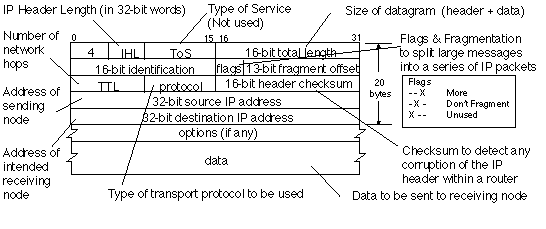
\includegraphics[width=6.8in]{IMAGES/headersections}
         \caption{Header Sections}
      \end{figure}

      \end{itemize}


\end{frame}

\cprotect\note{

}

\begin{frame}
   {TCP/IP and OSI Models}
      \begin{figure}[H]
         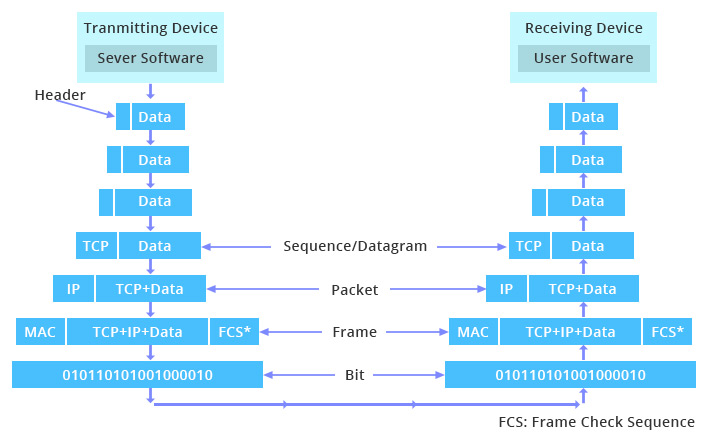
\includegraphics[width=6.0in]{IMAGES/models}
         \caption{Network Models Sections}
      \end{figure}

\end{frame}

\cprotect\note{

}

\begin{frame}
   {IPv4 and IPv6 Addresses}
      \begin{itemize}
	      \item \textbf{ip addr show}
      \end{itemize}
      \begin{raw}
1: lo: <LOOPBACK,UP,LOWER_UP> mtu 65536 qdisc noqueue state UNKNOWN group 
	      default qlen 1000
    link/loopback 00:00:00:00:00:00 brd 00:00:00:00:00:00
    inet 127.0.0.1/8 scope host lo
       valid_lft forever preferred_lft forever
    inet6 ::1/128 scope host
       valid_lft forever preferred_lft forever
2: wlp1s0: <BROADCAST,MULTICAST,UP,LOWER_UP> mtu 1500 qdisc mq state UP 
	      group default qlen 1000
    link/ether 94:65:9c:7b:cd:a7 brd ff:ff:ff:ff:ff:ff
    inet 192.168.200.175/24 brd 192.168.200.255 scope global dynamic 
	      noprefixroute wlp1s0
       valid_lft 82501sec preferred_lft 82501sec
    inet6 fe80::54df:86ab:b128:11ef/64 scope link noprefixroute
       valid_lft forever preferred_lft forever

      \end{raw}

\end{frame}

\cprotect\note{

}

